\clearpage
\section{Umsetzung}
\subsection{Benutzerführung}
Die Applikation wurde so als Konsolenapplikation angelegt, dass alle Module auch einzeln verwendet werden können. Für Enduser wurde jedoch im \lstinline$starter.py$ ein Konsolen-gesteuerter Workflow implementiert.

\begin{enumerate}
	\item Titel für die Suche muss eingegeben werden
	\item Der Benutzer wird gefragt, ob er bereits vorhandene Twitterdaten analysieren will oder ob er neue Twitterdaten über das API herunterladen möchte.
	\begin{enumerate}
		\item Wenn der Benutzer neue Twitterdaten laden möchte wird er nach Schlüsselwörtern gefragt
		\item Dem Benutzer werden die eingegebenen Schlüsselwörter nochmals angezeigt und er muss bestätigen damit das API angestossen wird
		\item Die Daten werden heruntergeladen und im File \lstinline$keyword1_keyword2_...keywordn_raw_search_timestamp.txt$ abgelegt. Der Filepfad wird zurückgegeben.
	\end{enumerate}
	\item Wenn der Benutzer vorhandene Twitterdaten analysieren möchte, muss er den Pfad zum Twitterdatenfile angeben
	\item Der Benutzer bestätigt, dass er die Twitter Datenanalyse für die gegebenen Tweets starten möchte
	\item Das Programm analysiert die Daten, erstellt die Plots und ein Logfile mit Resultaten
\end{enumerate}

Live sieht dies wie in Abbildung \ref{fig:benutzerfuehrung} aus.

\begin{figure}[h]
  \centering
  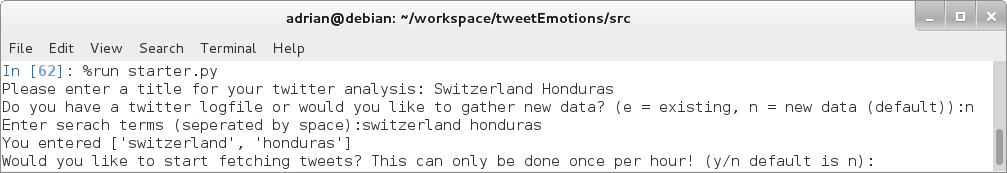
\includegraphics[width=0.8\textwidth]{images/benutzerfuehrung.png}
  \caption[Benutzerführung]{Benutzerführung}
  \label{fig:benutzerfuehrung}
\end{figure}

\subsubsection{Verwendete bzw. Eingebundene Ressourcen}
\begin{table}[H]
\begin{center}
\begin{tabular}{|l|l|}
	\hline
	\lstlisting$starter.py$ & Enthält den Code der Benutzerführung \\ \hline
	\lstlisting$gather_twitterdata.py$ & Enthält die Methoden zum herunterladen der Tweets \\ \hline
	\lstlisting$analyse_twitterdata.py$ & Wird mit MPI angestossen um die Daten zu analysieren \\ \hline
\end{tabular}
\caption{Verwendete Ressourcen: Benutzerführung}
\end{center}
\end{table}


\subsection{Twitterdaten Sammeln}
Wie bereits im Kapitel \ref{subsec:grundlagentwitter} beschrieben wurde zum Herunterladen der Tweets das Package TwitterSearch von Christian Koepp\cite{twittersearch} verwendet. 


\subsection{Algorithmen zur Erkennung der Gefühlslage in Texten}
\subsubsection{Emoticons}
\subsubsection{SentiWordNet}
\subsubsection{SenticNet}
\subsubsection{SASA}
\subsubsection{NLTK naive Bayes}
\subsection{Parallelisierung}